\chapter{Технологический раздел}
\section{Выбор средств реализации программного обеспечения}
Программное обеспечение состоит из трех модулей: модуль выделения информативных признаков сигнала, модуль кластеризации и модуль создания и обучения скрытых марковских моделей. 

Для модулей кластеризации и работы со скрытыми марковскими моделями был выбран язык Golang~\cite{golang}, поскольку процедура кластеризации и обучения скрытых марковских моделей предполагают работу с большими объемами данных. Golang имеет низкие накладные расходы на работу с памятью, что обеспечивает эффективную обработку с большими объемами данных.

Модуль выделения информативных признаков в основном содержит работу с аудиофайлами, поэтому для реализации этого модуля был выбран язык Python~\cite{python}. Python имеет широкий спектр библиотек и инструментов для обработки звуковых сигналов, в том числе и для выделения мел-кепстральных коэффициентов.

Для хранения и передачи данных между модулями было решено использовать реляционную базу данных. В качестве СУБД была выбрана PostgreSQL~\cite{postgresql}, поскольку языки Python и Golang, используемые для написания программного обеспечения, имеют встроенные пакеты работы с данной СУБД.

В качестве средства развертывания программного обеспечения была выбрана утилита Docker \cite{docker}, поскольку она поддерживает микросервисную архитектуру: Docker обеспечивает возможность разделения приложения на отдельные сервисы, которые могут быть запущены в отдельных контейнерах. 

%\subsection{Выбор СУБД}
%Для хранения и передачи данных между модулями было решено использовать реляционную базу данных. В качестве СУБД была выбрана PostgreSQL~\cite{postgresql}, поскольку языки Python и Golang, используемые для написания программного обеспечения, имеют встроенные пакеты работы с данной СУБД.
\section{Компоненты программного обеспечения} 
\subsection{Формирование вектора информативных признаков}
Компонент формирования вектора информативных признаков выполняет три основные задачи:
\begin{itemize}
	\item чтение файла разметки, предоставленного разработчиками корпуса DUSHA;
	\item формирование вектора мел-кепстральных коэффициентов для каждого кадра аудиофайла, прочитанного из файла разметки;
	\item запись информации об аудиофайлах, их кадрах и векторах мел-кепстральных коэффициентов в базу данных.
\end{itemize}
Задача чтения файла разметки выполняется классом DatasetProcessor, представленном на листинге \ref{lst:feature:dataset-processor}. В качестве аргументов конструктору класса предоставляется абсолютный путь до корпуса DUSHA в файловой системе компьютера и название файла, содержащего разметку.
\begin{lstlisting}[
	caption={Класс для чтения файла разметки},
	label=lst:feature:dataset-processor,
	language=Python]
class DatasetProcessor:
	def __init__(self, dataset_path, dataset_meta_file):
		self._dataset_path = dataset_path
		self._dataset_meta_file = dataset_meta_file
	
		self.wavs = []
		self._get_wavs()
	
	def _get_wavs(self):
		os.chdir(self._dataset_path)
		with open(self._dataset_meta_file, 'r') as mf:
			raw_data = list(mf)
			for i, rec in enumerate(raw_data):
				json_string = json.loads(rec)
				json_string["audio_path"] =
					_resolve_absolute_path(json_string["audio_path"])
				self.wavs.append(json_string)
\end{lstlisting}
Метод \_get\_wavs извлекает из файла разметки пути до аудиофайлов корпуса для дальнейшей работы с ними. В файле разметки присутствует относительный путь от самого файла разметки до аудиофайла корпуса, поэтому для чтения файла необходимо воссановить абсолютный путь аудиофайла корпуса. Это делает функция \_resolve\_absolute\_path.

После того, как пути были извлечены из файла разметки, требуется обработать каждый аудиофайл -- открыть его, разделить на кадры и вычислить мел-кепстральные коэффициенты для каждого кадра аудиофайла. Для работы с аудиофайлами реализован модельный класс сущности <<Аудиофайл>>, представленный на листинге \ref{lst:feature:sample} и модельный класс сущности <<Кадр>>, представленный на листинге \ref{lst:feature:frame}.
\begin{lstlisting}[
	caption={Модельный класс сущности <<Аудиофайл>>},
	label=lst:feature:sample,
	language=Python]
class Sample:
    def __init__(self, uuid, audio_path, emotion, batch):
        self.uuid = uuid
        self.audio_path = audio_path
        self.emotion = emotion
        self.batch = batch

    def __dict__(self):
        return {
            "uuid": self.uuid,
            "audio_path": self.audio_path,
            "emotion": self.emotion,
            "batch": self.batch
        }
\end{lstlisting}

\begin{lstlisting}[
	caption={Модельный класс сущности <<Кадр>>},
	label=lst:feature:frame,
	language=Python]
class Frame:
    def __init__(self, sample_id, index, mfcc):
        self.id = str(uuid.uuid4())
        self.sample_id = sample_id
        self.sample_num = index
        self.mfcc = mfcc
\end{lstlisting}

Класс AudioFeaturesExtractor (листинг \ref{lst:feature:extractor}) выполняет функции разделения аудиофайла на кадры и вычисления мел-кепстральных коэффициентов для каждого кадра аудиофайла.
\begin{lstlisting}[
	caption={Класс для формирования вектора информативных признаков},
	label=lst:feature:extractor,
	language=Python]
class AudioFeaturesExtractor:
    def __init__(self, file_path, frame_length=0.02, hop_length=0.01):
        sig, self.sampling_rate = librosa.load(file_path)
        self.frame_length = int(self.sampling_rate * frame_length) 
        self.hop_length = int(hop_length * self.sampling_rate)     
        self.frames = librosa.util.frame(sig, frame_length=
			self.frame_length, hop_length=self.hop_length)

    def get_mfcc(self, n_mfcc=13):
        mfcc = []
        for frame in self.frames.T:
            mfcc_per_frame = librosa.feature.mfcc(y=frame, sr=
				self.sampling_rate, n_fft=self.frame_length, n_mfcc=n_mfcc)
            mfcc.append(mfcc_per_frame.T)

        return np.array(mfcc)
\end{lstlisting}
При обработке аудиофайла (чтение, деление на кадры и извлечение мел-кепстральных коэффициентов) была использована библиотека <<Librosa>> \cite{librosa}, предназначенная для анализа и обработки аудиофайлов. 

Аргументами конструктора класса являются путь до аудиофайла в памяти компьютера, длина кадра и размер перекрытия. Метод get\_mfcc используется для извлечения вектора мел-кепстральных коэффициентов. Его аргументом является количество извлекаемых коэффициентов.

Класс SampleRepository (листинг \ref{lst:feature:sample-repo}) реализует <<репозиторий>> сущности <<аудиофайл>>, инкапсулирующий способ хранения данных.
\begin{lstlisting}[
	caption={<<Репозиторий>> сущности <<Аудиофайл>>},
	label=lst:feature:sample-repo,
	language=Python]
class SampleRepository(Repository):
    def __init__(self, db_client):
        self.db_client = db_client

	def create_many(self, entities):
        cursor = self.db_client.cnx.cursor()
        query = "INSERT INTO sample (uuid, audio_path, emotion, batch) 
			VALUES (%s, %s, %s, %s)"
        values = [(entity.uuid, entity.audio_path, entity.emotion,
			 entity.batch) for entity in entities]
        cursor.executemany(query, values)
        self.db_client.cnx.commit()
        cursor.close()

    def get(self):
        cursor = self.db_client.cnx.cursor()
        query = "SELECT uuid, audio_path, emotion, batch FROM sample"
        cursor.execute(query)

        samples = []
        for row in cursor.fetchall():
            uuid, audio_path, emotion, batch = row
            sample = Sample(uuid, audio_path, emotion, batch)
            samples.append(sample)

        cursor.execute(query)
        self.db_client.cnx.commit()
        cursor.close()

        return samples
\end{lstlisting}
Аналогично для сущности <<Кадр>> на листинге \ref{lst:feature:frame-repo} представлен класс FrameRepository, реализующий <<репозиторий>> сущности.
\begin{lstlisting}[
	caption={<<Репозиторий>> сущности <<Кадр>>},
	label=lst:feature:frame-repo,
	language=Python]
class FrameRepository(Repository):
    def __init__(self, db_client):
        self.db_client = db_client

        def _create_frames(self, frames):
        cursor = self.db_client.cnx.cursor()
        query = "INSERT INTO frame (uuid, sample_uuid, index)
			VALUES (%s, %s, %s)"
        values = [(frame.id, frame.sample_id, frame.sample_num)
			for frame in frames]
        cursor.executemany(query, values)
        self.db_client.cnx.commit()
        cursor.close()

    def _create_mfccs(self, frame_ids, mfccs):
        cursor = self.db_client.cnx.cursor()
        query = "INSERT INTO mfcc (uuid, frame_uuid, index, value)
			VALUES (%s, %s, %s, %s)"
        values = []
        for frame_id, mfcc in zip(frame_ids, mfccs):
            for i, c in enumerate(mfcc):
                mfcc_uuid = str(uuid.uuid4())
                value = c.item()
                values.append((mfcc_uuid, frame_id, i + 1, value))
        cursor.executemany(query, values)
        self.db_client.cnx.commit()
        cursor.close()

    def create_many(self, frames):
        frame_ids = [frame.id for frame in frames]
        mfccs = [frame.mfcc for frame in frames]

        self._create_frames(frames)
        self._create_mfccs(frame_ids, mfccs)
\end{lstlisting}
%Компонент формирования вектора информативных признаков представляет из себя веб-сервер, принимающий HTTP-запросы. Когда клиентское приложение обращается через метод <<POST>> на конечную точку <<\textit{/api/v1/samples}>>, сервер выполняет функцию чтения аудиофайлов из файла разметки, затем формирует векторы мел-кепстральных коэффициентов для каждого прочитанного аудиофайла и производит запись полученного набора векторов в базу данных для дальнейшего его использования другими компонентами ПО.

\subsection{Кластеризация}
Сервис кластеризации выполняет две основные задачи: кластеризация векторов информативных признаков и запись информации о кластерах и их центроидах в базу данных.

Функция KMeans, представленная на листинге \ref{lst:cluster:kmeans} в качестве входных данных принимает массив векторов информативных признаков каждого кадра каждого аудиофайла и возвращает массив центроидов кластеров, соответствующих этому набору.
\begin{lstlisting}[
	caption={Функция нахождения центроидов кластеров},
	label=lst:cluster:kmeans]
type Node []float64
	
func KMeans(Nodes []Node, clusterCount int, maxRounds int) ([]Node, error) {
	if len(Nodes) < clusterCount {
		return nil, 
		errors.New("amount of nodes is smaller than cluster count")
	}
	
	stdLen := 0
	for i, Node := range Nodes {
		curLen := len(Node)
		
		if i > 0 && len(Node) != stdLen {
			return nil, errors.New("data is not consistent dimension-wise")
		}
		stdLen = curLen
	}
	
	centroids := make([]Node, clusterCount)
	r := rand.New(rand.NewSource(time.Now().UnixNano()))
	for i := 0; i < clusterCount; i++ {
		srcIndex := r.Intn(len(Nodes))
		srcLen := len(Nodes[srcIndex])
		centroids[i] = make(Node, srcLen)
		copy(centroids[i], Nodes[r.Intn(len(Nodes))])
	}
	
	return initialCentroids(Nodes, maxRounds, centroids), nil
}
\end{lstlisting}
Для создания общего массива векторов информативных признаков каждого кадра необходимо извлечь их из базы данных. 

Для работы с кадрами аудиофайла реализована модельная структура сущности <<кадр>> (листинг  \ref{lst:cluster:frame}). Полям структуры присвоены json-метки, указывающие на соответствие полей структуры полям таблицы кадров в базе данных.
\begin{lstlisting}[
	caption={Модельная структура сущности <<кадр>>},
	label=lst:cluster:frame]
type Frame struct {
	ID           string `db:"uuid"`
	SampleUUID   string `db:"sample_uuid"`
	Index        int    `db:"index"`
	ClusterIndex string `db:"cluster_uuid"`
	MFCCs        []float64
}
\end{lstlisting}
Сущность <<кадр>> имеет соответствующую сервисную структуру (листинг \ref{lst:cluster:sample-service}), в которой присутствует функция, реализующая извлечение кадров из базы данных и функция, AssignCluster, которая ставит в соответствие кадру аудиофайла ближайший кластер.
\begin{lstlisting}[
	caption={Сервисная структура сущности <<кадр>>},
	label=lst:cluster:sample-service]
type FrameService struct {
	repo *postgres.FramePostgres
}

func (s *FrameService) GetAll() ([]entity.Frame, error) {
	frames, err := s.repo.GetAll()
	if err != nil {
		return nil, err
	}
	return frames, nil
}

func (s *FrameService) AssignCluster(frame entity.Frame, 
clusters []entity.Cluster) error {
	centroids := make([]kmeans.Node, len(clusters))
	for i, cluster := range clusters {
		centroids[i] = cluster.Centroid.Value
	}
	nearestIndex := kmeans.Nearest(frame.MFCCs, centroids)
	nearest := clusters[nearestIndex]
	
	return s.repo.AssignCluster(nearest.ID, frame.ID)
}
\end{lstlisting}
Структура FramePostgres, экземпляр которой присутсвует в поле сервисной структуры FrameService, реализует <<Репозиторий>> сущности <<кадр>>,  инкапсулирующий работу с базой данных Postgresql. Структура репозитория сущности <<Кадр>> представлена на листинге \ref{lst:cluster:frame-repo}.
\begin{lstlisting}[
	caption={Репозиторий сущности <<Кадр>>},
	label=lst:cluster:frame-repo]
type FramePostgres struct {
	db *sqlx.DB
}
\end{lstlisting}
Полем структуры является клиентское соединение с базой данных PostgreSQL. Репозиторий содержит метод GetAll, представленный на листинге \ref{lst:cluster:frame-repo-get-all}. В методе реализовано извлечение всех кадров и их информативных признаков из базы данных и помещает в соответствующий массив.
\begin{lstlisting}[
	caption={Извлечение кадров и их информативных признаков из базы данных},
	label=lst:cluster:frame-repo-get-all]
func (f *FramePostgres) GetAll() ([]entity.Frame, error) {
	var frames []entity.Frame
	
	query := `SELECT f.uuid, f.sample_uuid, f.index, 
	array_agg(m.value ORDER BY m.index) AS mfccs
	FROM frame f INNER JOIN mfcc m ON f.uuid = m.frame_uuid
	GROUP BY f.uuid, f.sample_uuid, f.index, f.cluster_uuid`
	
	rows, err := f.db.Query(query)
	if err != nil {
		return nil, err
	}
	
	for rows.Next() {
		var (
		uuid       string
		sampleUUID string
		index      int
		mfccsStr   string
		)
		err = rows.Scan(&uuid, &sampleUUID, &index, &mfccsStr)
		if err != nil {
			return nil, err
		}
		
		mfccs, err := parseMFCC(mfccsStr)
		if err != nil {
			return nil, err
		}
		
		frames = append(frames, entity.Frame{
			ID:         uuid,
			SampleUUID: sampleUUID,
			Index:      index,
			MFCCs:      mfccs,
		})
	}
	
	return frames, nil
}
\end{lstlisting}
После получения массива центроидов кластеров необходимо установить соответствие между кадром и кластером, к которому этот кадр принадлежит.  Кластер ставится в соответствие кадру в результате выполнения функции Nearest, представленной на листинге \ref{lst:cluster:nearest}.
\begin{lstlisting}[
	caption={Функция находления ближайшего кластера},
	label=lst:cluster:nearest]
func Nearest(in Node, nodes []Node) int {
	count := len(nodes)
	
	results := make(Node, count)
	
	cnt := make(chan int)
	for i, node := range nodes {
		go func(i int, node, cl Node) {
			results[i] = distance(in, node)
			cnt <- 1
		}(i, node, in)
	}
	
	wait(cnt, results)
	
	minI := 0
	curDist := results[0]
	
	for i, dist := range results {
		if dist < curDist {
			curDist = dist
			minI = i
		}
	}
	
	return minI
}
\end{lstlisting}
Функция Nearest оперирует индексами центроидов. При дальнейшей работе используется не целочисленный индекс кластера, а соответствующие ему модельные структуры сущности <<кластер>> и сущности <<центроид>>. Модельная структура сущности <<кластер>> представлена на листинге \ref{lst:cluster:cluster-centroid}.
\begin{lstlisting}[
	caption={Модельные структуры сущностей <<кластер>> и <<центроид>>},
	label=lst:cluster:cluster-centroid]
type Cluster struct {
	ID       string   `db:"uuid"`
	Index    int      `db:"index"`
	Centroid Centroid `db:"centroid_id"`
}

type Centroid struct {
	ID    string    `db:"uuid"`
	Value []float64 `db:"value"`
}
\end{lstlisting}

Для записи данных о кластере в базу так же имеется соответствующий репозиторий, аналогичный репозиториям остальных сущностей. 

Установка соответствия между центроидом кластера и его модельной структурой Cluster реализована в функции constructClusterData сервисного класса ClusterService, представленной на листинге \ref{lst:cluster:cluster-cluster-data}.
\begin{lstlisting}[
	caption={Установка соответствия между центроидом кластера и его модельной структурой},
	label=lst:cluster:cluster-cluster-data]
func (s *ClusterService) constructClusterData(centroids []entity.Centroid) 
[]entity.Cluster {
	clusters := make([]entity.Cluster, len(centroids))
	
	for i, centroid := range centroids {
		clusters[i] = entity.Cluster{
			ID:       uuid.New().String(),
			Index:    i + 1,
			Centroid: centroid,
		}
	}
	return clusters
}
\end{lstlisting}
Аналогичная функция представлена для установки соответствия между индексом центроида и его модельной структурой Centroid (листинг \ref{lst:cluster:cluster-centroid-data}).
\begin{lstlisting}[
	caption={Установка соответствия между индексом центроида и его модельной структурой},
	label=lst:cluster:cluster-centroid-data]
func (s *ClusterService) constructCentroidsData(centroidsCoords
[]kmeans.Node) []entity.Centroid {
	centroids := make([]entity.Centroid, len(centroidsCoords))
	
	for i, centroid := range centroidsCoords {
		centroids[i] = entity.Centroid{
			ID:    uuid.New().String(),
			Value: centroid,
		}
	}
	
	return centroids
}
\end{lstlisting}
В методе AssignClusters сервисного класса ClusterService, представленном на листинге \ref{lst:cluster:cluster-assign-clusters}, реализована кластеризация векторов информативных признаков. Метод возвращает массив модельных структур полученных кластеров.
\begin{lstlisting}[
	caption={Кластеризация},
	label=lst:cluster:cluster-assign-clusters]
func (s *ClusterService) AssignClusters(frames []entity.Frame, 
nclusters, maxRounds int) ([]entity.Cluster, error) {
	nodes := s.collectFramesData(frames)
	
	centroidsCoords, err := kmeans.KMeans(nodes, nclusters, maxRounds)
	if err != nil {
		return nil, err
	}
	
	centroids := s.constructCentroidsData(centroidsCoords)
	return s.constructClusterData(centroids), nil
}
\end{lstlisting}

\subsection{Создание и обучение скрытых марковских моделей}
Компонент создания и обучения скрытых марковских моделей выполняет три функции:
\begin{itemize}
	\item создание марковской модели для каждой эмоции;
	\item обучение каждой скрытой марковской модели;
	\item распознавание эмоций в аудиофайлах.
\end{itemize}
На листинге \ref{lst:ml:hmm-struct} представлена структура скрытой марковской модели, где <<Transitions>> -- матрица переходов, <<Emissions>> -- матрица эмиссий и <<StationaryProbabilities>> -- вектор начальных состояний.
\begin{lstlisting}[
	caption={Модельная структура скрытой марковской модели},
	label=lst:ml:hmm-struct]
type HiddenMarkovModel struct {
	Transitions             [][]float64 `json:"transitions"`
	Emissions               [][]float64 `json:"emissions"`
	StationaryProbabilities []float64   `json:"stationary_probabilities"`
}
\end{lstlisting}
Обучение скрытой марковской модели с использованием алгоритма Баума~---~Велша основано на принципе EM (\textit{англ. expectation-maximization}), поэтому изначально матрицы скрытой марковской модели инициализируются случайным образом (Е-этап).

На листинге \ref{lst:ml:hmm-init} представлена случайная инициализация матриц скрытой марковской модели.
\begin{lstlisting}[
	caption={Инициализация скрытой марковской модели},
	label=lst:ml:hmm-init]
func New(nStates, nObs int) *HiddenMarkovModel {
	seed := rand.New(rand.NewSource(0))
	emitProb := allocateRandomMatrix(nStates, nObs, seed)
	transProb := allocateRandomMatrix(nStates, nStates, seed)
	initProb := make([]float64, nStates)
	sum := 0.0
	for i := range initProb {
		initProb[i] = seed.Float64()
		sum += initProb[i]
	}
	for i := range initProb {
		initProb[i] /= sum
	}
	
	return &HiddenMarkovModel{
		Transitions:             transProb,
		Emissions:               emitProb,
		StationaryProbabilities: initProb,
	}
}
\end{lstlisting}

Для обучения скрытой марковской модели требуется прочитать данные об аудиофайлах и их кадрах из базы данных. В модельной структуре сущности <<кадр>> (листинг \ref{lst:ml:frame}) присутствуют не значения мел-кепстральных коэффициентов, а индексы кластеров, к которым принадлежит соответствующий набор значений мел-кепстральных коэффициентов. 
\begin{lstlisting}[
	caption={Модельная структура сущности <<кадр>>},
	label=lst:ml:frame]
type Frame struct {
	ID           string `db:"uuid"`
	SampleID     string `db:"sample_uuid"`
	Index        int    `db:"frame_index"`
	ClusterIndex int    `db:"cluster_index"`
}
\end{lstlisting}
Модельная структура сущности <<аудиофайл>> представлена на листинге \ref{lst:ml:sample}. 
\begin{lstlisting}[
	caption={Модельная структура сущности <<аудиофайл>>},
	label=lst:ml:sample]
type Sample struct {
	ID        string `db:"uuid"`
	AudioPath string `db:"audio_path"`
	Emotion   Label  `db:"emotion"`
	Frames    []Frame
}
\end{lstlisting}

Создание последовательности наблюдаемых в аудиофайле кластеров осуществляется в функции ConstructObservationSequence сервисного класса SampleService (листинг \ref{lst:ml:construct-obs}). В дальнейшем эта последовательность будет использована как входные данные для алгоритмов обучения и распознавания.

\begin{lstlisting}[
	caption={Создание последовательности наблюдений},
	label=lst:ml:construct-obs]
func (s *SampleService) ConstructObsSequence(sm entity.Sample) []int {
	observations := make([]int, len(sm.Frames))
	for i := 0; i < len(observations); i++ {
		observations[i] = sm.Frames[i].ClusterIndex - 1
	}
	return observations
}
\end{lstlisting}
В языке программирования Go операции числа с плавающей запятой представляются в виде научной нотации. Когда происходит умножение двух очень маленьких чисел, может произойти недостаточное представление точности числа с плавающей запятой. Поэтому все операции с вероятностями марковской модели происходят в логарифмической шкале.
Процедура прямого прохода  представлена на листинге \ref{lst:ml:forfard}.
\begin{lstlisting}[
	caption={Процедура прямого прохода},
	label=lst:ml:forfard]
func (hmm *HiddenMarkovModel) ForwardAlgorithm(obs []int,
alpha [][]float64) float64 {
	for i := 0; i < len(hmm.Transitions); i++ {
		alpha[0][i] = math.Log(hmm.StationaryProbabilities[i]) +
		math.Log(hmm.Emissions[i][obs[0]])
	}
	for t := 1; t < len(obs); t++ {
		for j := 0; j < len(hmm.Transitions); j++ {
			sum := math.Inf(-1)
			for i := 0; i < len(hmm.Transitions); i++ {
				sum = logAdd(sum, alpha[t-1][i] + 
				math.Log(hmm.Transitions[i][j]))
			}
			alpha[t][j] = sum + math.Log(hmm.Emissions[j][obs[t]])
		}
	}
	logLikelihood := math.Inf(-1)
	for i := 0; i < len(hmm.Transitions); i++ {
		logLikelihood = logAdd(logLikelihood, alpha[len(obs)-1][i])
	}
	return logLikelihood
}
\end{lstlisting}
Процедура обратного прохода представлена на листинге \ref{lst:ml:backward}. 
\begin{lstlisting}[
	caption={Процедура обратного прохода},
	label=lst:ml:backward]
func (hmm *HiddenMarkovModel) BackwardAlgorithm(obs []int, 
								beta [][]float64) {
	for i := 0; i < len(hmm.Transitions); i++ {
		beta[len(obs)-1][i] = 0.0
	}
	
	for t := len(obs) - 2; t >= 0; t-- {
		for i := 0; i < len(hmm.Transitions); i++ {
			logSum := math.Inf(-1)
			
			for j := 0; j < len(hmm.Transitions); j++ {
				logSum = logAdd(logSum,
				math.Log(hmm.Transitions[i][j]) + 
				math.Log(hmm.Emissions[j][obs[t+1]])+beta[t+1][j])
			}
			
			beta[t][i] = logSum
		}
	}
}
\end{lstlisting}
Вычисление $\gamma$-вероятностей представлен на листинге \ref{lst:ml:gamma}.
\begin{lstlisting}[
	caption={Вычисление $\gamma$-вероятностей},
	label=lst:ml:gamma]
func (hmm *HiddenMarkovModel) computeGamma(obs []int, alpha [][]float64, 
								beta [][]float64, gamma [][]float64) {
	for t := 0; t < len(obs); t++ {
		sum := math.Inf(-1)
		
		for i := 0; i < len(hmm.Transitions); i++ {
			gamma[t][i] = alpha[t][i] + beta[t][i]
			sum = logAdd(sum, gamma[t][i])
		}
		
		for i := 0; i < len(hmm.Transitions); i++ {
			gamma[t][i] -= sum
			gamma[t][i] = math.Exp(gamma[t][i])
		}
	}
}
\end{lstlisting}
Вероятности $\alpha$, $\beta$ и $\gamma$ используются при вычислении $\xi$-вероятностей, использующихся при корректировке матриц скрытой марковской модели в алгоритме Баума~---~Велша. Вычисление $\xi$-вероятностей представлено на листинге  \ref{lst:ml:xi}.
\begin{lstlisting}[
	caption={Вычисление $\xi$-вероятностей},
	label=lst:ml:xi]
func (hmm *HiddenMarkovModel) computeXi(obs []int, alpha [][]float64, 
								beta [][]float64, xi [][][]float64) {
	for t := 0; t < len(obs)-1; t++ {
		for i := 0; i < len(hmm.Transitions); i++ {
			for j := 0; j < len(hmm.Transitions); j++ {
				xi[t][i][j] = alpha[t][i] + math.Log(hmm.Transitions[i][j])+
				math.Log(hmm.Emissions[j][obs[t+1]]) + beta[t+1][j]
			}
		}
	}
	
	for t := 0; t < len(obs)-1; t++ {
		maxVal := math.Inf(-1)
		
		for i := 0; i < len(hmm.Transitions); i++ {
			for j := 0; j < len(hmm.Transitions); j++ {
				if xi[t][i][j] > maxVal {
					maxVal = xi[t][i][j]
				}
			}
		}
		
		sum := 0.0
		
		for i := 0; i < len(hmm.Transitions); i++ {
			for j := 0; j < len(hmm.Transitions); j++ {
				xi[t][i][j] = math.Exp(xi[t][i][j] - maxVal)
				
				sum += xi[t][i][j]
			}
		}
		
		for i := 0; i < len(hmm.Transitions); i++ {
			for j := 0; j < len(hmm.Transitions); j++ {
				xi[t][i][j] /= sum
			}
		}
	}
}
\end{lstlisting}
Алгоритм Баума~---~Велша, выполняющий корректировку матриц модели (M-этап принципа EM), принимает в качестве входных данных массив индексов кластеров (наблюдаемых состояний) и количество итераций корректирования матриц. 

Обучение скрытой марковской модели с использованием алгоритма Баума~---~Велша представлено на листинге \ref{lst:ml:baum-welch}.
\begin{lstlisting}[
	caption={Алгоритм Баума~---~Велша},
	label=lst:ml:baum-welch]
func (hmm *HiddenMarkovModel) BaumWelch(observationSequence []int,
iterations int) {
	var (
	alpha = make([][]float64, len(observationSequence))
	beta  = make([][]float64, len(observationSequence))
	gamma = make([][]float64, len(observationSequence))
	xi    = make([][][]float64, len(observationSequence)-1)
	)
	
	for i := 0; i < len(observationSequence); i++ {
		alpha[i] = make([]float64, len(hmm.Transitions))
		beta[i] = make([]float64, len(hmm.Transitions))
		gamma[i] = make([]float64, len(hmm.Transitions))
		
		if i < len(observationSequence)-1 {
			xi[i] = make([][]float64, len(hmm.Transitions))
			
			for j := 0; j < len(hmm.Transitions); j++ {
				xi[i][j] = make([]float64, len(hmm.Transitions))
			}
		}
	}
	
	hmm.Emissions = LaplaceSmoothing(hmm.Emissions)
	
	for it := 0; it < iterations; it++ {
		hmm.ForwardAlgorithm(observationSequence, alpha)
		hmm.BackwardAlgorithm(observationSequence, beta)
		hmm.computeGamma(observationSequence, alpha, beta, gamma)
		hmm.computeXi(observationSequence, alpha, beta, xi)
		
		// Update the model parameters
		hmm.update(observationSequence, gamma, xi)
	}
}
\end{lstlisting}

Для избежания появления нулей в матрице эмиссий скрытой марковской модели перед первой итерацией алгоритма Баума~---~Велша следует использовать сглаживание. В качестве метода сглаживания был выбран метод сглаживания Лапласа \cite{smooting}.
%
Сглаживания Лапласа заключается в добавлении к каждому элементу матрицы эмиссий некоторого малого значения. В данном случае к каждому элементу строки добавляется единица и затем каждая строка матрицы нормализуется. Функция, выполняющая сглаживание Лапласа, представлена на листинге \ref{lst:ml:smoothing}.
\begin{lstlisting}[
	caption={сглаживание Лапласа},
	label=lst:ml:smoothing]
func LaplaceSmoothing(emissionMatrix [][]float64) [][]float64 {
	rows := len(emissionMatrix)
	cols := len(emissionMatrix[0])
	
	smoothedMatrix := make([][]float64, rows)
	
	for i := 0; i < rows; i++ {
		smoothedMatrix[i] = make([]float64, cols)
		for j := 0; j < cols; j++ {
			smoothedMatrix[i][j] = (emissionMatrix[i][j] + 1) /
			(sum(emissionMatrix[i]) + float64(cols))
		}
	}
	return smoothedMatrix
}
\end{lstlisting}
Обученные марковские модели решено хранить в JSON-файле. Функция записи матриц скрытой марковской модели в файл представлена на листинге \ref{lst:ml:save-json}.
\begin{lstlisting}[
	caption={Запись матриц скрытой марковской модели в файл},
	label=lst:ml:save-json]
func (hmm *HiddenMarkovModel) SaveJSON(filename string) error {
	file, err := os.Create(filename)
	if err != nil {
		return err
	}
	defer file.Close()
	
	encoder := json.NewEncoder(file)
	if err := encoder.Encode(hmm); err != nil {
		return err
	}
	return nil
}
\end{lstlisting}

Наиболее вероятную эмоцию можно получить после запуска алгоритма прямого хода. В нем вычисляется вероятность наблюдать представленную на вход алгоритма последовательность, при условии заданной модели. Эта вероятность называется вероятностью наблюдения. Вычисление вероятности наблюдения представлено на листинге \ref{lst:ml:forfard} в строках 17-22.

Из вычисленных вероятностей наблюдения выбирается максимальная. Скрытая марковская модель, которой принадлежит максимальная вероятность наблюдения считается подходящей для входной последовательности и эмоция, на которой была обучена эта модель, считается наиболее вероятной.

Результат распознавания эмоций представлен в качестве матрицы несоответствий. На листинге \ref{lst:ml:cm} представлена инициализация матрицы несоответствий с использованием истинных и спрогнозированных значений разметки.
\begin{lstlisting}[
	caption={Инициализация матрицы несоответствий},
	label=lst:ml:cm]
func NewConfusionMatrix(labels []entity.Label, actual,
predicted []entity.Label) *ConfusionMatrix {
	confusionMatrix := make(map[entity.Label]map[entity.Label]float64)
	for _, ac := range labels {
		confusionMatrix[ac] = make(map[entity.Label]float64)
		for _, pred := range labels {
			confusionMatrix[ac][pred] = 0.
		}
	}
	for i := 0; i < len(actual); i++ {
		confusionMatrix[actual[i]][predicted[i]]++
	}
	return &ConfusionMatrix{labels: labels, Values: confusionMatrix}
}
\end{lstlisting}
Матрицу несоответствий перед отображением следует нормализовать. Нормализованная матрица несоответствий обычно представляется в виде долей. На листинге \ref{lst:ml:cm-norm} представлена нормализация матрицы несоответствий.
\begin{lstlisting}[
	caption={Нормализация матрицы несоответствий},
	label=lst:ml:cm-norm]
func (m *ConfusionMatrix) Normalize() {
	numClasses := len(m.labels)
	rowSums := make([]float64, numClasses)
	totalSum := 0.0
	for i, actualLabel := range m.labels {
		for _, predictedLabel := range m.labels {
			rowSums[i] += m.Values[actualLabel][predictedLabel]
			totalSum += m.Values[actualLabel][predictedLabel]
		}
	}
	normConfusionMatrix := make(map[entity.Label]map[entity.Label]float64)
	for i, actualLabel := range m.labels {
		normConfusionMatrix[actualLabel] = make(map[entity.Label]float64)
		for _, predictedLabel := range m.labels {
			normConfusionMatrix[actualLabel][predictedLabel] = 
			m.Values[actualLabel][predictedLabel] / rowSums[i]
		}
	}
	m.Values = normConfusionMatrix
}
\end{lstlisting}


\section{Тестирование компонент программного обеспечения}
Для оценки правильности работы программного обеспечения было проведено тестирование алгоритма обучения скрытой марковской модели. Было выделено три класса эквивалентности, представленных в таблице \ref{tab:eq-test}.

\begin{table}[H]
	\centering
	\caption{Классы эквивалентности}\label{tab:eq-test}
	\begin{tabular}{|O|T|P|T|}
		\hline
		\textit{№} & \textit{Описание} & \textit{Входные данные} & \textit{Ожидаемый результат} \\ \hline
		1 & входная последовательность наблюдаемых состояний содержит различные состояния & эмиссии, наблюдаемые состояния & алгоритм правильно откорректирует матрицу эмиссий \\ \hline
		2 & входная последовательность наблюдаемых состояний содержит одно и то же состояние & эмиссии, наблюдаемые состояния & алгоритм правильно откорректирует матрицу эмиссий \\ \hline
		3 & На вход алгоритму подается 2500 состояний & количество состояний & в результирующей матрице эмиссий не встретится ни одного значения NaN \\ \hline
	\end{tabular}
\end{table}
NaN (\textit{англ. Not a Number}) -- значение, представленное типом данных float64 в языке Golang. Оно появляется когда выполняются математические операции, которые не могут быть корректно вычислены или не имеют определенного значения. В случае алгоритмов скрытой мароквской модели, NaN может появиться в матрице эмиссий в том случае, когда количество состояний велико, и, следовательно, вероятность нахождения модели в определенном состоянии настолько мала, что ее мантисса может потерять значимые цифры.

Для тестов 1-2 подготовлены файлы, содержащие значения матрицы эмиссиий и последовательности состояний. В случае теста 3 был подготовлен только файл, содержащий значения последовательности состояний, а сама матрица эмиссий задавалась случайным образом, поскольку проверка самих значений в тесте №3 не требуется. Процедура выполнения тестов 1-2 представлена на листинге \ref{lst:test:obs-wrapper}.
\begin{lstlisting}[
	caption={Выполнение  тестов №1-2},
	label=lst:test:obs-wrapper]
func TestHiddenMarkovModel_BaumWelch(t *testing.T) {
	testCases := []struct {
		name  string
		fEmit string
		fObs  string
		fExp  string
		dim   int
	}{
		{
			name:  "STATES DIFFER",
			fEmit: "etc/test-cases/hmm-diff-emit",
			fExp:  "etc/test-cases/hmm-diff-expect",
			fObs:  "etc/test-cases/hmm-diff-obs",
			dim:   50,
		},
		{
			name:  "SAME STATE",
			fEmit: "etc/test-cases/hmm-same-emit",
			fExp:  "etc/test-cases/hmm-same-expect",
			fObs:  "etc/test-cases/hmm-same-obs",
			dim:   50,
		},
	}
	
	for _, testCase := range testCases {
		t.Run(testCase.name, func(t *testing.T) {
			err := runBaumWelchTest(testCase.fEmit, testCase.fObs, 
			testCase.fExp, testCase.dim)
			if err != nil {
				t.Fatal(err)
			}
		})
	}
}
\end{lstlisting}
Каждый тестовый случай представлен структурой в массиве testCases, в которой присутствует название теста (поле name), файл с матрицей эмиссий (поле fEmit), файл с массивом наблюдаемых состояний (поле fObs), файл с ожидаемым значением матрицы эмиссий после прогона алгоритма (поле fExp) и размерность матрицы эмиссий (поле dim). Тестовый прогон алгоритма Баума~--- ~Велша представлен на листинге \ref{lst:test:bw}.
\begin{lstlisting}[
	caption={Тестовый прогон алгоритма Баума~---~Велша},
	label=lst:test:bw]
func runBaumWelchTest(fEmit, fObs, fExp string, dim int) error {
	emit, err := readMatrixFromFile(fEmit, 1, dim)
	if err != nil {
		return err
	}
	hmm := HiddenMarkovModel{
		Transitions: [][]float64{
			{1},
		},
		Emissions:               emit,
		StationaryProbabilities: []float64{1},
	}
	obs, err := readArrayFromFile(fObs)
	if err != nil {
		return err
	}
	hmm.BaumWelch(obs, 1)
	expectedEmissions, err := readMatrixFromFile(fExp, 1, dim)
	if err != nil {
		return err
	}
	equal := matricesEqual(hmm.Emissions, expectedEmissions, 0.005)
	if !equal {
		return errors.New("emission matrix differs from expected")
	}
	return nil
}
\end{lstlisting}
Выполнение теста №3 представлено на листинге \ref{lst:test:bw-nan}.
\begin{lstlisting}[
	caption={выполнение теста №3},
	label=lst:test:bw-nan]
func TestHiddenMarkovModel_BaumWelchBigMatrix(t *testing.T) {
	dim := 2500
	model := New(1, dim)
	obs, err := readArrayFromFile("_meta/test-cases/hmm-big-obs")
	if err != nil {
		t.Fatal(err)
	}
	model.BaumWelch(obs, 100)
	if hasNaN(model.Emissions) {
		t.Fatal(fmt.Errorf("matrix has NaN values"))
	}
}
\end{lstlisting}

\section{Формат входных и выходных данных}  
Компонент формирования вектора информативных признаков принимает на вход файл формата YAML \cite{yaml}, содержащий следующие поля:
\begin{itemize}
	\item <<dataset\_path>>: абсолютный путь к корневой директории корпуса речи;
	\item следующие поля для DSN (\textit{англ. Data Source Name}) строки соединения с базой данных:
	\begin{itemize}
		\item <<psql\_bind\_ip>>: сервер, на котором работает база данных;
		\item <<psql\_port>>: порт, на котором работает база данных;
		\item <<psql\_user>>: имя пользователя базы данных;
		\item <<psql\_password>>: пароль для пользователя базы данных;
		\item <<psql\_database>>: имя базы данных.
	\end{itemize}
\end{itemize}
Так же компонент принимает на вход параметр командной строки <<dataset\_metafile>>, представляющий относительный путь файла разметки от корневой директории корпуса речи <<dataset\_path>> и параметр <<mode>>, представляющий ключ для выполняемого действия: <<from-file>>, если требуется заполнить базу данных из файла разметки и <<add>>, если требуется добавить файл по его абсолютному пути. Во втором случае принимается на вход также аргумент <<audio\_path>>, представляющий собой абсолютный путь до файла, подвергаемого обработке.

Компонент кластеризации так же принимает на вход файл формата YAML, содержащий следующие поля:
\begin{itemize}
	\item Аналогичные конфигурационному файлу для компонента формирования вектора информативных признаков поля для DSN строки соединения с базой данных (<<psql\_bind\_ip>>, <<psql\_port>>, <<psql\_user>>, <<psql\_password>>, <<psql\_database>>) и параметр <<ssl\_mode>>, определяющий уровень требуемой безопасности для соединения;
	\item <<cluster\_amount>>: число кластеров для алгоритма k-means;
	\item <<kmeans\_max\_rounds>>: число итераций для алгоритма k-means.
\end{itemize}
Так же компонент принимает на вход параметр командной строки <<mode>>, представляющий ключ для выполняемого действия: <<cluster-all>>, если требуется произвести кластеризацию всех кадров в базе данных, и <<assign>> в случае если требуется соотнести один набор кадров с соответствующими кластерами. Во втором случае принимается на вход также аргумент <<audio\_path>>, представляющий собой абсолютный путь до файла, подвергаемого обработке.

Компонент создания и обучения скрытых марковских моделей принимает на вход параметр командной строки <<mode>>, представляющий ключ для выполняемого действия (обучение, проверка или распознавание), принимающий значения <<test>>, <<train>> и <<recognize>>. Также компонент создания и обучения скрытых марковских моделей принимает на вход файл формата YAML, содержащий следующие поля:
\begin{itemize}
	\item Аналогичные конфигурационному файлу для компонента кластеризации поля для DSN строки соединения с базой данных;
	\item <<cluster\_amount>>: число кластеров алгоритма k-means (для задания количества состояний моделей);
	\item <<model\_file\_path>>: шаблон для имени файла скрытой марковской модели, представляющий строку со строковым спецификатором формата, в который во время выполнения алгоритма будет подставлено название эмоции.
\end{itemize}
Компонент создания и обучения скрытых марковских моделей имеет также выходной параметр -- html-файл, содержащий инструкции отображения матрицы ошибок в веб-браузере.

\section{Физические компоненты системы и их размещение на устройствах}
Система распознавания размещена на одном устройстве, однако для каждого компонента присутствует собственная среда исполнения: компоненты создания и обучения СММ и кластеризации имеют среду исполнения Golang, в то время как компонент формирования информативных признаков имеет среду исполнения Python3.  Точка входа, агрегирующая все функции системы, так же имеет свою среду исполнения.  Диаграмма развертывания, отражающая особенности физической архитектуры системы, представлена на рисунке \ref{fig:deploy}.
\begin{figure}[H]
	\centering
	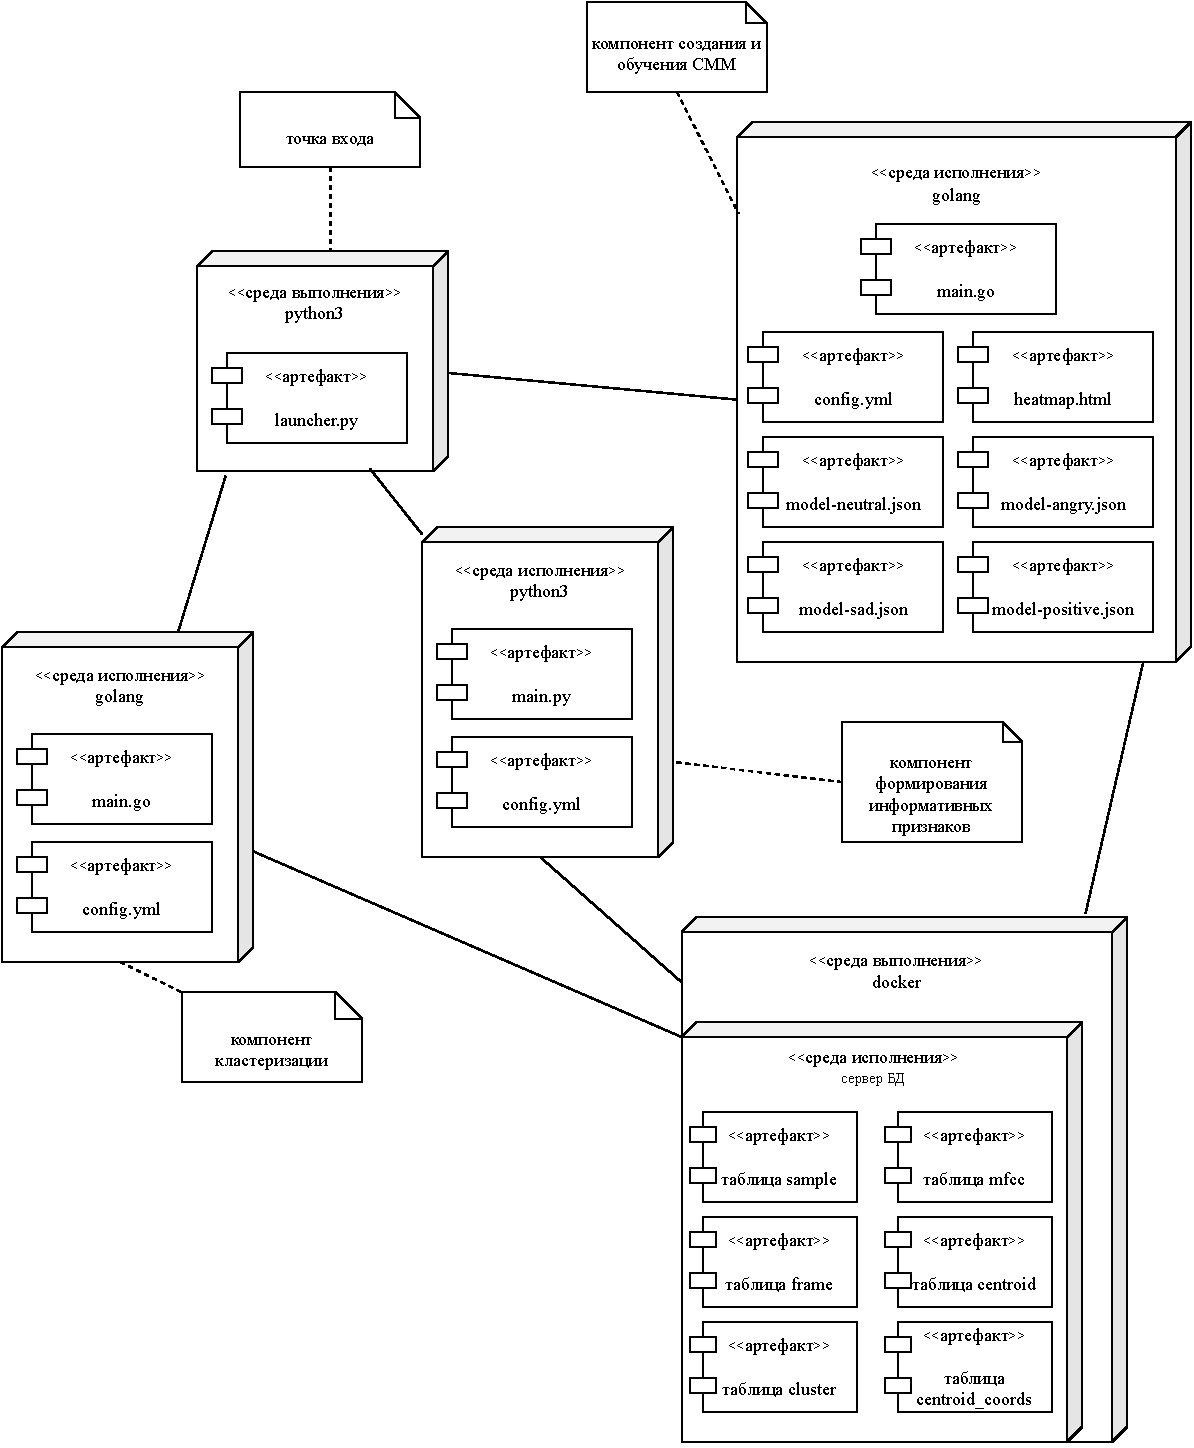
\includegraphics[width=\linewidth]{assets/deploy}
	\caption{Диаграмма развертывания}
	\label{fig:deploy}
\end{figure} 
